\documentclass[../main.tex]{subfiles}
\begin{document}
	This section contains all of the functional and quality requirements of the system. It gives a detailed description of the system and all its features.
	\section{External interface Requirements}
		This section provides a detailed description of all inputs into and outputs from the system. It also gives a description of the hardware, software and communication interfaces and provides basic prototypes of the user interface.
	\subsection{User interfaces}
		For each access users of the application should see the log-in page, to provide credentials and authenticate.
		\begin{figure}[h]
			\centering
			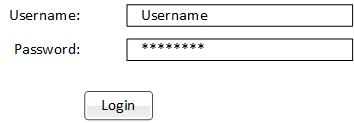
\includegraphics{login}
			\caption{Login page}
		\end{figure}\\
		When logged, users must be able to search practices and work on it. The open practices ordered by due date will listed once the user logged in successfully. He can choose to visualise the open, the closed, the suspended and all the practices using tabs as showed in figure.
		\begin{figure}[h]
			\centering
			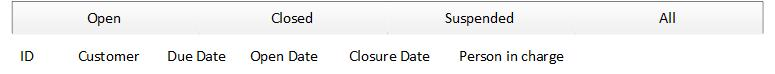
\includegraphics{home}
			\caption{Home page}
		\end{figure}\\
	\subsection{Hardware interfaces}
	\subsection{Software interfaces}
	\subsection{Communications interfaces}
	\section{Functional requirements}
		 This section includes the requirements that specify all the fundamental actions of the software system.
	\section{Performance requirements}
		The requirements in this section provide a detailed specification of the user interaction with the software and measurements placed on the system performance.
	\section{Design constraints}
		This section includes the design constraints on the software caused by the hardware.
	\section{Software system attributes}
		The requirements in this section specify the required reliability, availability, security and maintainability of the software system. 
\end{document}